\chapter{Intrinsic network architecture and its relationship to skilled reading}

\epigraph{Modularity in the organization of biological systems confers significant advantages in an evolutionary setting, by supporting adaptability and robustness and thus increasing the system's evolvability.}{Sporns \& Betzel\\\textit{Modular Brain Networks}}

\section{Motivation}

\begin{itemize}
    \item Resting-state fMRI is the first place to be studied, small-world architecture.
    \item Modular properties are known to exist. Some suggestion that they are related to individual differences 
    \item Not often paired with an exploration of methods. Validate connectomics methods - does it fit our sample of developing readers?
    \item There is the further question of whether these skills are sensitive to reading only. Are any measures related to reading skill? What is the best way to measure this? Are multiple measures sensitive? There is clear support for this idea in the literature: whole-brain measures of architecture have correlated with intelligence and psychiatric disorders. However, reading presents a unique opportunity to focus on a variety of skills.
    \item Are there RSN-level trends in how networks are related?
    \item In this chapter, we would like to establish what relationship, if any,  intrinsic network architecture has with individual differences in reading. First, we validate the existence of a small-world architecture in these subjects, and that the network parcellation is appropriate for them. Second, we determine whether global measures of interconnectedness, including modularity, participation coefficient and path length, are related to reading skill. Finally, we investigate which resting-state networks or brain regions drive the relationship between connectivity and reading skill. In particular, we are interested in whether this might be apparent through resting-state fMRI, which can be performed before children even start reading.
\end{itemize}


% Skilled reading requires the coordination of many skills, including those encompassing visual recognition and oral language comprehension (Hoover & Gough, 1990), and even, as is increasingly being recognized, executive processes (Aboud, Bailey, Petrill, & Cutting, 2016; Cartwright, 2012; Cutting et al., 2009). Consequently, reading requires the integration of various cognitive processes across many brain regions. More specifically, the brain areas underlying reading involve a substantial number of left-hemisphere regions (Price, 2012), with supporting functions contributed by right hemisphere homologues (Lindell, 2006). The left occipito-temporal cortex in particular is a region whose activation increases with reading skill (Cohen et al., 2000); activation in this region becomes more lateralized as individuals’ reading abilities progress and also distinguishes typically developing readers from impaired ones (Turkeltaub et al., 2003; van der Mark et al., 2009). Over development it is thought that the occipito-temporal region tunes to graphical features, such as letters, which then provide a new modality of input to extant language systems, including regions of the left inferior frontal gyrus and temporo-parietal cortices (Schlaggar & McCandliss, 2007). 

A number of studies have investigated the differences between skilled and impaired readers. In general, skilled reading is associated with left hemisphere language and word recognition regions (left inferior frontal, supramarginal and occipito-temporal regions), and fronto-parietal regions supporting attention (Paulesu, Danelli, & Berlingeri, 2014). Understanding how their coordination at rest relates to variability in reading ability is of interest. 

The brain regions supporting reading do not, however, form a unique, fundamental network. Instead, reading appears to rely on the reconfiguration and integration of multiple, more fundamental brain networks (Koyama et al., 2010; Vogel et al., 2013). One way in which brain networks have been identified is by the correlated activation of brain regions over time during rest.  These so-called resting-state networks (RSNs) are distinct over time and composed of brain regions that tend to function as a unit (De Luca et al., 2006; Smith et al., 2009; Yeo et al., 2011; among others). This functional division into networks is hypothesized to provide a neural substrate for the diversity of cognitive functions in which people engage (Yeo et al., 2014). Examination of these networks can be done noninvasively using functional magnetic resonance imaging even when participants are not engaged in specific cognitive processes and are at rest (Fox & Raichle, 2007). 
% Depending on specifics of the methodology, studies across thousands of individuals suggest that on average the brain segregates into 7-17 RSNs (Damoiseaux et al., 2006; Yeo et al., 2011). These networks resemble those evoked from task-based fMRI (Smith et al., 2009), and so are commonly assigned labels based on function (e.g., ventral attention network). 

While these networks generally are thought to be highly similar across people (Damoiseaux et al., 2006), individual variations in the intensity or spatial extent of RSNs have been noted. For example, differences have been observed in individuals who exhibit variation in cognitive ability (e.g., Reineberg et al., 2015; Tian et al., 2013) and in individuals with genetic susceptibility to Alzheimer’s disease (e.g., Filippini et al., 2009). Moreover, the patterns of RSN activity within an individual is consistent over periods of time in excess of three years (Choe et al., 2015). It is thought that this stability may reflect a history of co-activation among brain regions that occurs over time (Power et al., 2010). As such, variation in RSNs are likely to be stable measures of individual differences. To date, however, their relationship to other cognitive domains, and in particular reading, is not well understood.  Given that we know broad scale networks underlie a variety of cognitive functions, it follows that individual variation within certain reading-related networks and the interaction among RSNs could be linked to varying reading abilities. The existence of these associations can be used to not only predict cognitive and academic functioning at the level of the individual, but also aid treatment allocation or prediction of developmental trajectory (e.g., Mattfeld et al., 2014) or response-to-intervention (e.g., Crowther et al., 2015; Whitfield-Gabrieli et al., 2015). 

Indeed, emerging research suggests that functional connectivity indices are associated with differences in reading skill. Struggling readers, such as those with dyslexia, exhibit decreased connectivity between visual association areas and prefrontal attention areas, increased right hemisphere connectivity, and reduced connectivity to occipito-temporal cortex compared to non-impaired readers (Finn et al., 2014).  In typically developing readers, Koyama and colleagues (2011) found increased positive connectivity among language regions was associated with increased word reading ability, and recent studies suggest that interventions designed to enhance reading skill can increase the correlations between visual and frontal executive areas (Horowitz-Kraus, Toro-Serey, & Difrancesco, 2015). It is therefore likely that fast and efficient readers have coordinated neural systems that include both traditional language areas, as well as broader, more domain general networks.  

Although most cognitive functions are relevant to reading in some way, the RSNs most associated with primary reading subprocesses are the frontoparietal, ventral attention, and visual RSNs.  In addition to the intensity of and specific spatial composition of these networks, coordination between these brain areas and others are also likely to play a role in differentiating higher from lower performing individuals. For example, Koyama et al., 2011 found that increased reading ability was associated with increased negative connectivity between reading regions and regions of the default mode network, a network typically implicated in internally-directed thinking/mentation (Andrews-Hanna, 2011). This negative relationship between the default and reading networks echoes work showing that increased anti-correlated activity between the default network and regions specialized for cognitive function, such as those involved in attention (Kelly et al., 2008; Mennes et al., 2010; Seeley et al., 2007), inhibitory control (Tian et al., 2013), and working memory (Keller et al., 2015; Sala-Llonch et al., 2011) is associated with individuals who display higher performance.

An in depth examination of how behavioral indices of reading relate to various properties of RSNs has not been previously reported, especially in a large sample. Here we investigate ...

% how variation in the intensity or spatial extent of RSNs containing classic language and reading areas relates to individual differences in reading during the adolescence and young adulthood (range: 13.5-20.5). We also consider the relationships between RSNs, bearing in mind the possibility that individual differences in reading ability could be driven by interaction among reading areas and networks with complementary or opposing cognitive function such as the default RSN. For example, increased negative connectivity between reading-related and default RSNs in skilled readers could indicate beneficial segregation or insulation of reading-related cognitive processing from the influence of self-referential/autobiographical processes usually associated with default network function. Thus, we explore the relationships of different RSNs to each other based on the temporal correlation of their time courses, expecting that, consistent with previous findings showing increased cognitive functioning is associated with task positive RSNs being more negatively correlated to the default RSN, skilled readers will show stronger negative correlations between these same, or similar, RSNs than their less skilled peers.




\section{Methods}

The following methods detail the current study's protocol and analytic approach. The following chapters borrow heavily from the methods described below, so they are explained here in detail. 

\subsection{Participants}

Participants were drawn from the fourth wave of a larger, longitudinal study investigating the neurobiological bases of reading comprehension. 52 children completed scans and a subset of these met the motion and attention thresholds described below.

All participants were native English speakers with normal hearing and normal or corrected vision, and no history of major psychiatric illness or traumatic brain injury/epilepsy. Subjects had no history of a developmental disability or contra-indication to MRI.  Each participant gave written consent at the beginning of the study, with procedures carried out in accordance with Vanderbilt University’s Institutional Review Board.

\begin{table}
    \renewcommand{\tabcolsep}{0.09cm}
    \centering
    \begin{tabular}{lc}
\toprule 
Measure & Subjects \\ 
\midrule 
No. Participants				& 42 \\ 
No. Scan Runs					& 164 \\ 
Gender  						& 25 F \\ 
Age at Scan 					& 10.5 (0.3)  \\ 
WASI Full-Scale IQ  			& 111.0 (16.2) \\ 
TOWRE - Total Word Efficiency 	& 104.6 (18.5) \\ 
\bottomrule 
\end{tabular}
    \caption[Participant demographics]{Demographics and mean test scores for Study 1 participants are described here. For continuous data, the standard deviation is enclosed in parentheses.}
    \label{table:ch2-participants}
\end{table}

In addition to having an MRI scan, participants completed cognitive tests, including the Wechsler Abbreviated Scale of Intelligence (WASI) \citep{Kaplan1999}, the Test of Word Reading Efficiency (TOWRE) \citep{Torgesen2012}, the Woodcock Reading Master Tests (WRMT) \citep{Woodcock1998}, and the Gates-MacGinitie Reading Comprehension test \citep{MacGinitie2000}. Demographics and selected test data are summarized in Table \ref{table:ch2-participants}.

\subsection{MRI acquisition and preprocessing}

Imaging was performed on a Philips Achieva 3T MR scanner with a 32-channel head coil. Functional images were acquired using a gradient echo planar imaging sequence with 40 (3 mm thick) slices with no gap. Resting-state fMRI scans consisted of 150 dynamic volumes. Slices were parallel to the anterior-posterior commissure plane. Imaging parameters for functional images included: TE = 30 ms; FOV = 240 x 240 x 120 mm\textsuperscript{3}; flip angle = 75\degree; TR = 2200 ms; and 3 mm\textsuperscript{3} isotropic voxels.

\begin{figure}[t]
    \centering
    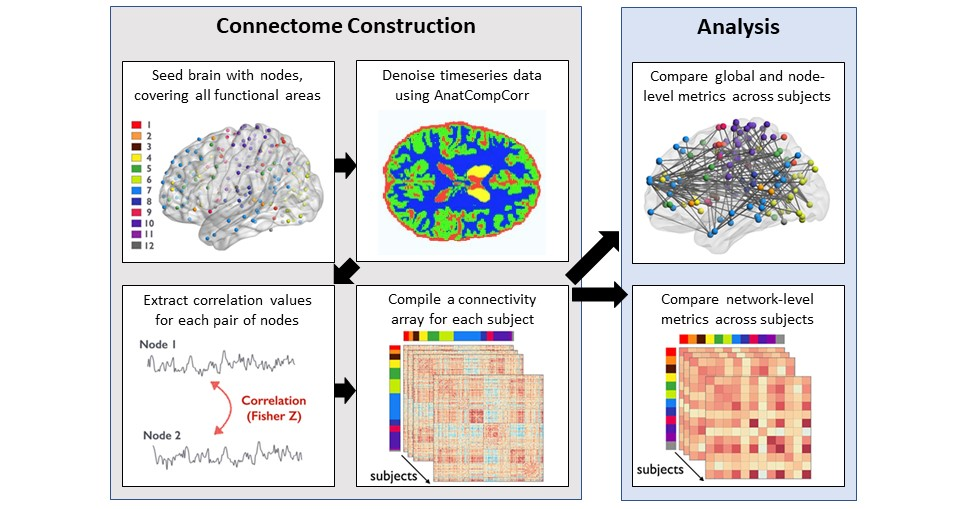
\includegraphics[width=6in]{ch2-connectome-methods}
    \caption[Schematic for connectome construction.]{Connectomes are constructed from resting-state fMRI in the following steps: slice-timing correction, rigid-body motion correction, boundary-based registration to a T1-weighted anatomical image, and normalization to MNI 152 template. The timseries for 264 nodes are then extracted and denoised using signal from non-neural tissue, continuous motion parameters and outliers. A pair-wise connectivity matrix is then calculated and thresholded at multiple different thresholds, then analyzed. Figure adapted from \citep{Yang2018}.}
    \label{fig:ch2-connectome-methods}
\end{figure}

Whole-brain fMRI analyses were performed using tools from the FMRIB Software Library (version 5.0.9). For each session, the following pre-processing steps were performed:  slice-time correction, motion correction to the initial fMRI volume, boundary-based registration to the subject's structural image, and normalization to 2 mm MNI 152 standard space. To mitigate the effects of motion on our analyses, we regressed out 6 continuous motion parameters and scrubbed out outlier volumes. We defined an outlier volume as any in which the root-mean-square framewise displacement exceeded 0.7 mm. Because head motion can be a major confound for connectivity analyses, we removed scan runs where more than 20 percent of the fMRI volumes were outliers.

\subsection{Connectome construction}

To investigate whole-brain patterns of connectivity with minimal investigator bias, we selected 264 nodes \textit{a priori} whose connectivity properties have been extensively analyzed in previous works \citep{Power2011}. The node set samples the entire brain, and nodes were selected based on their involvement in a diversity of cognitive tasks. Each node was assigned to one of 13 RSNs based on previous literature \citep{Power2013}. Approximately 10 percent of the nodes did not have a stable assignment in the original paper; for the present analyses, these nodes were excluded from graph theory calculations. A description of the 13 networks and their sizes is provided in \ref{table:ch2-power-nodes}. 

\begin{table}
	\renewcommand{\tabcolsep}{0.09cm}
	\centering
	\begin{tabular}{lcc}
\toprule 
Suggested RSN & Abbreviation & Nodes \\ 
\midrule 
\textit{Sensory} & & \\
	\hspace{3pt}Auditory  			&  AUD & 13 \\ 
	\hspace{3pt}Somatomotor (Hand)	&  SOH & 30 \\
	\hspace{3pt}Somatomotor (Mouth)	&  SOM & 5 \\
	\hspace{3pt}Visual	 			&  VIS & 31 \\ 
\textit{Attention} & & \\
	\hspace{3pt}Dorsal attention  	&  DAN & 11	\\ 
	\hspace{3pt}Salience		  	&  SAL & 18 \\ 
	\hspace{3pt}Ventral attention  	&  VAN & 9 \\ 
\textit{Executive / Associative} & & \\
	\hspace{3pt}Cingulo-opercular 	& CON & 14 \\ 
	\hspace{3pt}Default mode		& DMN & 58 \\
	\hspace{3pt}Fronto-parietal  	& FPN & 25 \\ 
	\hspace{3pt}Memory retrieval	& MEM & 5 \\
\textit{Other} & & \\
	\hspace{3pt}Cerebellar			& CER & 4  \\
	\hspace{3pt}Subcortical			& SUB & 13 \\
	\hspace{3pt}Not assigned 		& UNC & 28 \\ 
\bottomrule 
\end{tabular}
	\caption[List of networks.]{List of networks used in connectivity analyses and the number of nodes affiliated with each. Although alternative parcellations of the node set are possible, we elected to use those network assignments suggested in \citep{Power2013}.}
	\label{table:ch2-power-nodes}
\end{table}

Connectivity analysis was performed in the CONN toolbox \citep{WhitfieldGabrieli2012}. fMRI data were high-pass filtered at 0.008 Hz, motion-corrected, co-registered to a structural image, normalized to MNI space and smoothed by a 5 mm FWHM spherical kernel. Outlier volumes were identified as individual fMRI volumes in which the RMS framewise-displacement exceeded 0.7. fMRI timeseries were corrected using anatCompCorr methods, which uses signal from white matter tissue and cerebrospinal fluid areas to reduce noise not related to brain activity \citep{Chai2012}. We also regressed out 12 continuous measures of motion were also included and all outlier timepoints. The timeseries was then high-pass filtered at 0.01 Hz. fMRI timeseries correlations were calculated between each of the the 264 nodes, resulting in a single connectivity array for each subject at each time point. Matrices were then thresholded into binary maps by keeping the top 5 percent of connections. (To confirm that this particular threshold did not unduly influence results, we swept results between thresholds at the top 2 percent to the top 10 percent of connections. No significant effect on the results was found.)

\subsection{Connectome analyses}

The metrics of interest were network \textit{modularity}, \textit{participation coefficient} and \textit{path length}. Modularity is high in networks where nodes within the same RSN are highly connected to each other but not elsewhere. The participation coefficient, on the other hand, is high when many nodes are connected to several different RSNs. Both of these metrics relate to the integration of information between RSNs. Path length describes the distance between any two nodes on the graph. This was calculated between every node, then summed up by RSN to create a measure of network distance. These properties, and their changes within our task, were investigated at the level of connectomes, RSNs and nodes. 

First, we establish the validity of the parcellation for evaluting network properties in this sample. At rest, we expect to see high modularity (greater than 0.1), low participation (less than 0.9), and a lower path length within RSNs than between them. We also expect to see moderate-sized correlations between measures, since each is measuring an aspect of network architecture related to distance between nodes.  

Next, we break each global measure down by RSN to determine how sub-systems differ in their network roles. For modularity, we report the total modularity contribution for each network. For participation coefficient and path length, we report the mean value within each network. We also investigate the measures obtained across the whole range of network-forming thresholds (retaining the top 2 to 10 percent of connections). We expect to see changes in the measures across thresholds, but ranked in a relatively stable order among the different RSNs. 

To determine the relationship between network measures and individual performance on cognitive assessments, we input each global metric into a general linear model with the Test of Word Reading Efficiency (TOWRE, total word efficiency (TWE) standard score). Models containing measures of mean framewise-displacement (motion) and the WASI Vocabulary measure were also assesed to ensure that effects were not driven by motion confounds or global measures of cognitive skill. We also examined whether there were differences in the modularity relationship between TOWRE subtests (sight word efficiency (SWE) and phonemic decoding efficiency (PDE)). 

To assess whether there was an RSN-level trend in the modularity-to-reading relationship, post-hoc analyses comparing network-level modularity values to TOWRE scores were also investigated. For each node, a correlation value was calculated between its modularity contribution and TOWRE TWE scores. To evaluate significance, RSN correlations were compared to a bootstrapped distribution of 5000 correlation values generated by sampling and totaling the modularities for a random set of nodes equal in size to the selected RSN. (For example, adding 31 random nodes for comparison to the visual network.)


\section{Results} 

Of the 52 subjects who completed resting-state fMRI scans, 44 met the scan quality criteria for inclusion. Connectome parcellations at the 5 percent threshold exhibited small-world properties: the mean modularity value was 0.264 (SD = 0.037), and the mean participation coefficient was 0.599 (0.052). Furthermore, the path length within RSNs was significantly lower than those between: within-community nodes took an average of 2.49 (0.141) steps to reach each other, whereas between-community nodes took an average of 3.06 (0.207) steps ($p$ \textless 0.001, two-sample $t$-test). Furthermore, a comparison of each metric against the others shows that, while there is overlap between the measures at the global level, there is substantial variability as well (Table \ref{fig:ch2-global-graph-theory-descriptions}).

\begin{figure}[t]
    \centering
    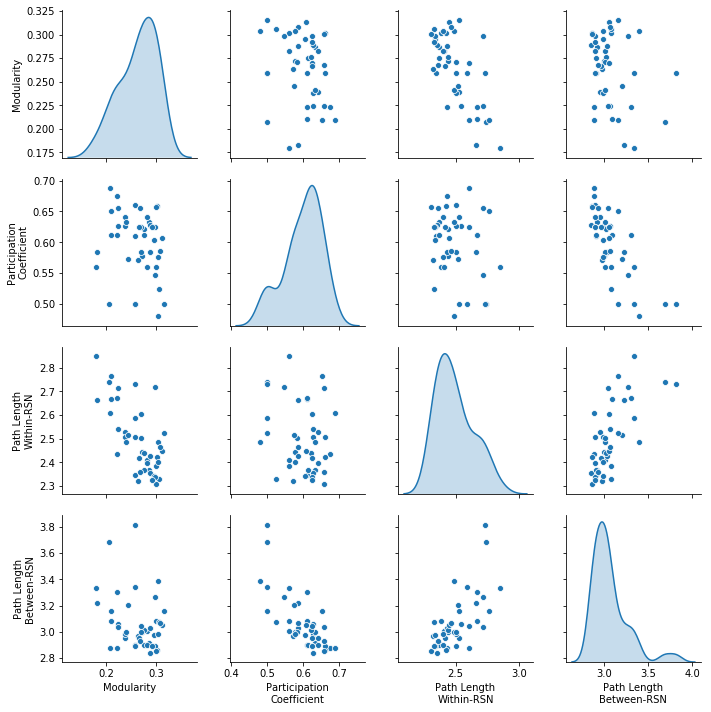
\includegraphics[width=5in]{ch2-global-graph-theory-descriptions}
    \caption[Distribution and correlations between global graph theory measures.]{Distribution and correlations between the global modularity, participation coefficient and path length. Each attribute may be interpreted as a measure of connectedness between RSNs, but there is significant variability between them.}
    \label{fig:ch2-global-graph-theory-descriptions}
\end{figure}

Figure \ref{fig:ch2-network-graph-theory-descriptions} highlights the contributions of each RSN to the graph theory measures. The visual, somatomotor, and default mode were the most modular RSNs, in part reflecting their larger size relative to others. The dorsal attention, auditory and cingulo-opercular networks were the most participatory RSNs at rest. The fronto-parietal RSN occupied an interesting place, possessing relatively high modularity but also one of the higher participation coefficients and lower global path lengths. The effect of changing thresholds had consistent effects on each measure: as more connections were included, the modularity decreased, participation coefficient increased, and path length decreased (Fig.  \ref{fig:ch2-network-graph-theory-descriptions}, bottom). 

\begin{figure}[t]
    \centering
    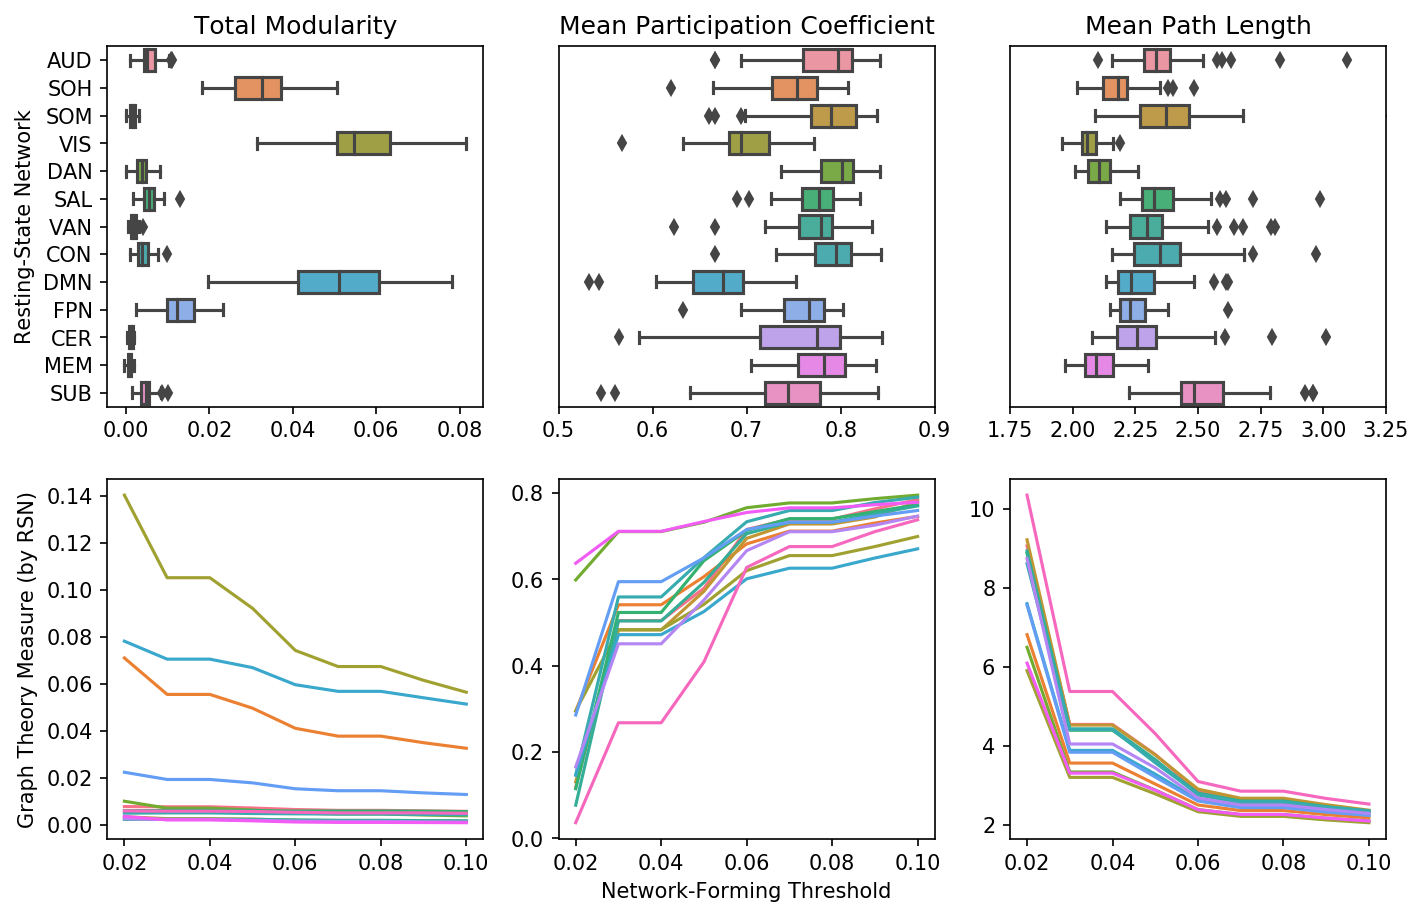
\includegraphics[width=6in]{ch2-network-graph-theory-descriptions}
    \caption[Relationships between network-level graph theory measures.]{Relationships between network-level graph theory measures. Shown above are the network-level distributions of the graph theory measures when graphs are thresholded for the top 10 percent of connections (top row), and the network means as the network-forming thresholds are swept from 2 percent to 10 percent (bottom row).}
    \label{fig:ch2-network-graph-theory-descriptions}
\end{figure}

The relationships between each graph theory metric to TOWRE are summarized in Table \ref{table:ch2-global-glm-results}. Global modularity, but not participation coefficient or path length, was predictive of reading skill even after controlling for mean framewise displacement (motion) and verbal intelligence ($Z_{TWE} = 2.536$). The direction of the relationship was positive, and it was higher for the ``sight word efficiency'' subtest than for ``phonemic decoding efficiency'' ($Z_{SWE} = 2.779$, $Z_{PDE} = 2.138$), which did not reach significance when confounds were controlled. 

\begin{table}[t]
    \renewcommand{\tabcolsep}{0.09cm}
    \centering
    \begin{tabular}{lcc}
\toprule 
Independent Variable & Coeff. & $p$-value \\ 
\midrule 
\textit{Sensory} & & \\
	\hspace{3pt}Auditory  			&  AUD & 13 \\ 
	\hspace{3pt}Somatomotor (Hand)	&  SOH & 30 \\
	\hspace{3pt}Somatomotor (Mouth)	&  SOM & 5 \\
	\hspace{3pt}Visual	 			&  VIS & 31 \\ 
\textit{Attention} & & \\
	\hspace{3pt}Dorsal attention  	&  DAN & 11	\\ 
	\hspace{3pt}Salience		  	&  SAL & 18 \\ 
	\hspace{3pt}Ventral attention  	&  VAN & 9 \\ 
\textit{Executive} & & \\
	\hspace{3pt}Cingulo-opercular 	& CON & 14 \\ 
	\hspace{3pt}Default mode		& DMN & 58 \\
	\hspace{3pt}Fronto-parietal  	& FPN & 25 \\ 
	\hspace{3pt}Memory retrieval	& MEM & 5 \\
\textit{Other} & & \\
	\hspace{3pt}Cerebellar			& CER & 4  \\
	\hspace{3pt}Subcortical			& SUB & 13 \\
	\hspace{3pt}Not assigned 		& UNC & 28 \\ 
\bottomrule 
\end{tabular}
    \caption{Results for analyses comparing global graph theory metrics to reading skill.}
    \label{table:ch2-global-glm-results}
\end{table}

The relationship between modularity and TOWRE is stable across multiple thresholds (Fig. \ref{fig:ch2-global-glm-covariates-thresh}). In fact, when graph theory measures were compared to other language-related assessments, there was a trend towards a significant positive relationship between modularity and cognitive performance that was more stable than those of either the participation coefficient or global path length. 

\begin{figure}[t]
    \centering
    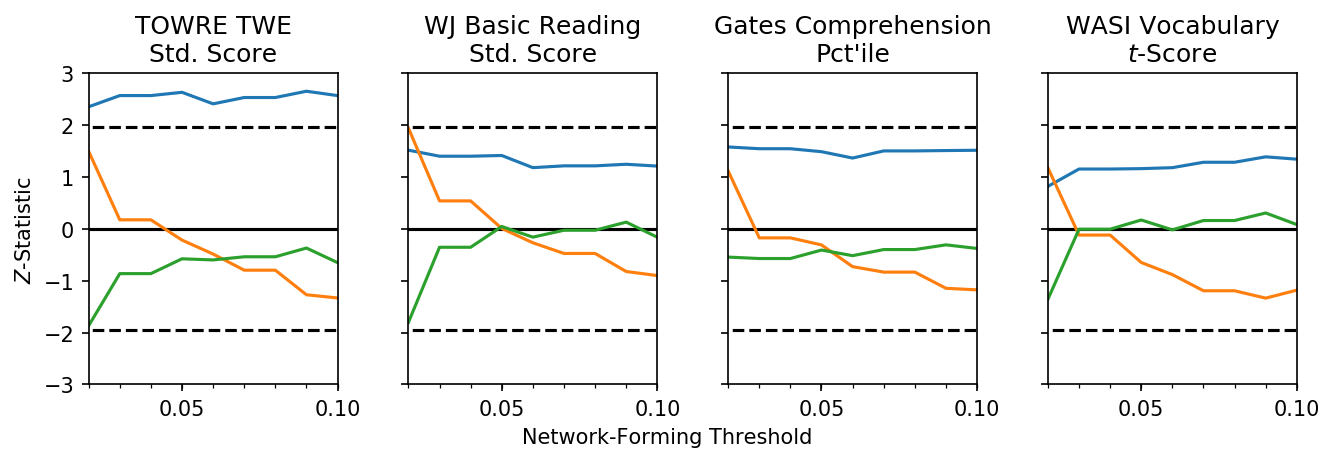
\includegraphics[width=5.5in]{ch2-global-glm-covariates-thresholds}
    \caption[Modularity metrics at rest are the best predictors of cognitive skills.] {Global modularity was the most stable and predictive network measure for predicting language-related skills, although it only reached significance thresholds for the TOWRE.}
    \label{fig:ch2-global-glm-covariates-thresh}
\end{figure}

Finally, we investigated the correlation between each individual RSN's modularity contribution and TOWRE scores (Fig. \ref{fig:ch2-rsn-node-modularity-corr}. Overall, no RSN reached the level of significance that the global modularity measure (i.e., $r = 0.378$). The default mode RSN had the highest correlation with the TOWRE ($r_{DMN} = 0.350$), with the memory retrieval ($r_{MEM} = 0.303$) and attention ($r_{DAN} = 0.236$, $r_{VAN} = 0.248$) RSNs ranking next. Although not significant, the relationship was inverted in the auditory RSN: lower modularity was associated with better reading skill ($r = -0.178$).

\begin{figure}[t]
    \centering
    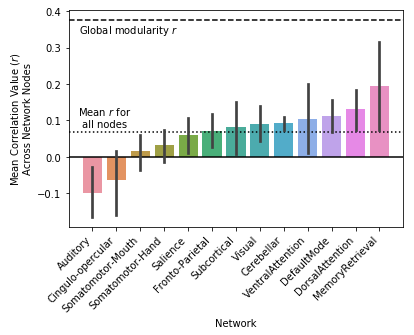
\includegraphics[height=3in]{ch2-rsn-node-modularity-corr}
    \caption[Modularity relationship with TOWRE varies by RSN.] {Modularity relationship with TOWRE varies by RSN. Although no RSN reached the level of significance that the global modularity measure, the default mode and memory retrieval RSNs had significant positive correlations with the TOWRE.}
    \label{fig:ch2-rsn-node-modularity-corr}
\end{figure}

\section{Discussion}

In this first section, we establish that resting-state fMRI can connect robustly to behavioral metrics of reading efficiency. Modularity, in particular, indexes these skills. This is consistent with previosu research: the degree of segregation is critically important at rest. 

The distribution of the modularity is equally important: we see theat certain networks provide a larger aomuont of modularity per node than others. 

How the connectome changes during reading is an important next step that we will tackle in the following chapter.

The current study found evidence that individual differences in the composition of RSNs are associated with reading ability.  More specifically, our results indicated that the frontoparietal RSN was expanded to right-hemisphere language areas in good readers. Poorer readers, in contrast, exhibited an expansion of the default-posterior RSN to lateral occipital and subcortical regions and expansion of the sensory-somatomotor RSN to middle temporal and frontal polar regions. Finally, we found the frontoparietal and default-posterior RSNs were more anti-correlated in more skilled readers.  We discuss the implications of each of these findings in more detail below.

\subsection{Validation of methodology}

Our analysis of overlap between ICA-derived RSNs in the present study and a meta-analysis of many task-based fMRI studies of reading showed overlap with two distinct networks: the frontoparietal and ventral attention RSNs.  This finding is consistent with previous studies, which have reported that there is no single “reading” resting-state network, but rather that reading functions are dispersed across multiple more fundamental networks (Vogel et al., 2013). Both RSNs are composed predominantly of higher-order association cortex.  

We found a relationship between reading ability and variation in the extent of one of the reading network analogs – the left frontoparietal RSN. Task-based neuroimaging provides us with a rich description of the functions of frontoparietal network. The frontoparietal network is an assembly of brain regions encompassing the lateral frontal and parietal cortices along with insular, anterior/mid cingulate, and inferior temporal areas that have been broadly implicated in a variety of higher-level cognitive tasks (Fedorenko, Duncan, & Kanwisher, 2013). Some have described the frontoparietal network as supporting active and adaptive online control, initiating and adjusting goal-directed mental systems (Dosenbach et al., 2007), while others have proposed a more general superordinate role in directing cognition (Niendam et al., 2012). The most obvious relationship of the frontoparietal network to language is its proximity to Broca’s area, known for its critical role in language articulation. Rather than thinking of this area (traditionally, Brodmann areas 44 and 45) as exclusively or primarily language-related, it has been argued that Broca’s area supports hierarchical executive processing, such as the segmentation (“chunking”) of auditory language and the flexible combination of words (Koechlin & Jubault, 2006). Thus, while Broca’s area plays a role in the unification of representations, prefrontal cortex (and the larger frontoparietal network) may play a higher-level control and initiating role in language and other processes (Hagoort, 2005). 

Our findings show that in stronger readers, the left frontoparietal RSN is expanded to include portions of the right posterior middle and superior temporal cortex.  These regions may play a number of roles in more skilled readers.  First, these right hemisphere regions are homologues of important left hemisphere language areas. The left posterior superior and middle temporal gyri are major secondary processing areas for written and auditory word stimuli (Price, 2012). In the right hemisphere, these areas are understood to play a complementary role, with a sensitivity to both emotional and prosodic elements (Jung-Beeman, 2005). Thus, the expansion of the frontoparietal network to these homologues could represent greater “recruitment” of complimentary language areas, facilitating  the integration of language-related information.  Secondly, these right hemisphere areas are subregions of the generally bilateral ventral attention RSN (Yeo et al., 2011).  Nonetheless in task-based studies, this network shows more of a right-sided bias (Fox et al., 2006).  As such, good readers may be better at integrating visual information with more high-order information.  These explanations need not be mutually exclusive.

While we found an expansion of the left frontoparietal RSN to regions of the ventral attention RSN in good readers, we did not find an association between variation in the ventral attention RSN itself and individual differences in reading ability. The ventral attention network detects salient or unexpected stimuli in the environment (Vossel, Geng, & Fink, 2014). In this way the ventral attention network can act as a ‘circuit breaker’ for the dorsal system to help reorient attention (Corbetta and Shulman, 2002). It may thus help orient individuals to new information from the visual environment (i.e. text) and, by coupling stimulus-driven attentional areas with the frontoparietal network, it may help construct updated mental representations of linguistic material. The leftward aspects of the ventral attention network underlie crucial reading-related areas, including occipito-temporal cortex, which performs orthographic processing, and temporo-parietal cortex, important for semantic binding (Taylor, Rastle, & Davis, 2013). The absence of reading-related variance associated with the entire bilateral RSN may reflect the diversity of functions that these areas serve in basic visual and auditory processing, as well as language and reading. 

\subsection{Connectome-level relationships to reading}

We also explored how the variation in other RSNs (i.e., those networks not primarily dedicated to reading-related functions) is associated with individual differences in reading ability. We found poorer readers showed expansions in two RSNs: the default-posterior RSN and the sensory-somatomotor RSN. The default-posterior RSN was expanded to a lateral occipital region as well as two subcortical areas in readers with low ability. The default-posterior RSN is notable because it contains the anterior hub of the default network – medial prefrontal cortex – an area that is both a core hub of the default network (in more anterior aspects; Andrews-Hanna et al., 2010)) as well as a crucial element of a default network subsystem that may be specialized for theory of mind and social processing (among other functions described in more detail in (Andrews-Hanna, 2011)). Although speculative, these expansions in poor readers could translate functionally to a network that is susceptible to interference. In the case of the poor readers in our study, typical medial prefrontal cortex functions that could be applied in reading contexts could be susceptible to interferences from functions associated with occipital cortex. In addition to the default-posterior expansion, poor readers also showed expansion of the sensory-somatomotor RSN to left frontal pole and left middle temporal gyrus. Taken together, these exploratory results suggest less cohesion of default-posterior and sensory-somatomotor RSNs may be an important neural correlate of poor reading ability, perhaps signaling a lack of balance between the segregation of various cognitive functions (i.e., altered functional modularity). Although expansion of the left frontoparietal, default-posterior, and sensory-somatomotor RSNs is related to reading ability, subsequent investigations should evaluate the extent to which these findings predict unique variance in reading ability above that of more traditional functional or structural indicators.

\subsection{Resting-state network-level relationships to reading}
}
    
We found increased reading ability was associated with more negative correlation between the time courses of the left frontoparietal and default-posterior RSNs. Although no consensus theoretical interpretation of frontoparietal to default correlations exists, one could speculate that increased negative correlations between the RSNs enables segregation of functions. This interpretation stems from a wide range of studies showing opposing activation in externally directed cognitive tasks for the frontoparietal and default RSNs, during which functions of the two networks ought to be segregated to prevent interference from the internal mentation functions of the default network. Our finding is notable for several reasons. This finding replicates previous work in many cognitive domains (including reading) that shows a cognitive advantage of increased negative connectivity between task-positive and task-negative RSNs while notably extending that work in both methodology and the specificity of the result. Regarding methodology, here we used a large sample to lessen concerns of possible correlation inflation induced by a small sample (Schönbrodt & Perugini, 2013). Additionally, our use of ICA-derived time courses for RSNs-of-interest lessens concerns that preprocessing choices could induce artifactual negative correlations between RSNs (Murphy et al., 2009). Regarding specificity, the age range of our sample of participants covers a unique developmental period between adolescence and young adulthood in which …  Additionally, the fractionation of the default network into anterior and posterior aspects in the ICA analysis allowed us to investigate the interaction of subcomponents of the default network and various task-positive RSNs. We found a unique result in that only the correlation between the left frontoparietal network and a network containing the posterior hub of the default network was associated with individual differences in reading ability. Posterior cingulate cortex is a major hub of the default network (Leech, Braga, & Sharp, 2012) with a proposed specific role in processing personal significance, introspection of preferences, feelings, and emotions, and evoked emotions (Andrews-Hanna et al., 2010). A separate line of work has shown the posterior cingulate cortex exhibits connectivity that is particularly well suited to influence frontal motor control areas (Uddin et al., 2009). Future work should consider possible differences in the correlations of task-positive RSNs to various subcomponents of the default network by either extracting the time courses of multiple default network regions (rather than medial prefrontal cortex as a default network proxy region alone) or pursuing a data-driven approach by allowing ICA to determine the network structure of the specific data set at hand. More generally, future work must establish the specific benefits of increased negative correlations between RSNs to skilled readers.

\subsection{Limitations}

While our study is one of the largest studies of the relationships between reading skills and intrinsic functional connectivity, it is not without limitations. One limitation is that we used a composite measure of reading. Since reading relies on a number of subordinate processes (e.g. word recognition and semantic processing), it is possible that our results do not reflect differences across specific domains relevant to reading and that such relationship might be observed. Another limitation is that, because we examined these relationships in relatively mature readers, it is possible that other relationships might be observed in developing readers. For example, our null findings for individual differences in the ventral attention RSN could reflect our sample’s relative maturity with respect to reading development since the ventral attention RSN overlaps with left hemisphere regions supporting lower-level reading processes such as orthographic processing. Such processes explain less and less variance in reading skill as texts become more difficult and reading starts to reach mature levels (Cutting et al., 2006). 

\subsection{Conclusion}

Overall, the current results are a powerful demonstration of the possibilities of using resting-state as a marker of individual differences.  We find that individual variations in RSNs are associated with overall reading proficiency.  More highly skilled readers recruit an expanded language network analog at rest, while poorer readers show expanded default and sensory-somatomotor RSNs and more cross-over between the default-posterior and frontoparietal RSNs, which has previously been associated with lower levels of cognitive performance in other non-reading domains. 
